\section{The Gaussian chain: diffusion breaks locality}
\label{sec:gaussian}

\begin{figure*}[t]
  \centering
  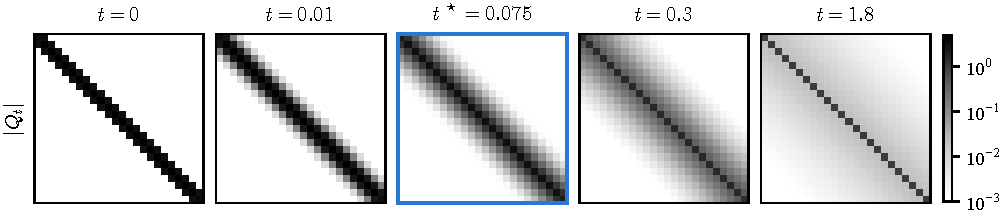
\includegraphics{fig_locality}
  \caption{\note{$|Q_t|$ of the Gaussian chain ($\alpha=0.85$, $L=24$) at $t=0$, $0.01$, $t^\star=0.075$, $0.3$,
  $1.8$: tridiagonal at $t=0$, densest at $t^\star$ (framed), diagonal at large $t$. Slide 5.}}
  \label{fig:locality}
\end{figure*}

\note{J\'er\^ome (12:01, 33:47): the denoiser is tridiagonal only for a while; diffusion breaks locality; so locality
cannot be had by stupidly fitting a tridiagonal matrix. Score $=-Q_tx$, $Q_t=(e^{-2t}\Sigma_0+\Delta_tI)^{-1}$.}

\note{Numbers: $t^\star=0.0753$ (generator printout). Best denoiser restricted to a window of radius $r$, Gaussian
chain, infinite data: relative score error $0.20$ ($r=1$), $0.089$ ($r=2$), $0.029$ ($r=4$), $0.0066$ ($r=8$)
--- thesis \texttt{fig\_ch10.windowed\_oracle}.}

\note{End: the posterior is still a chain; for the Gaussian chain inference on it is the Kalman smoother.}
